\chapter{Inégalités, Convergences et Théorème Limite}

\section{Inégalités de Probabilités}

Ces inégalités fournissent des bornes sur les probabilités sans connaître la loi exacte de la variable aléatoire, seulement certains de ses moments (comme l'espérance ou la variance).

\subsection{Inégalité de Markov}

Soit $X$ une variable aléatoire telle que $\E[|X|]$ existe et est finie. Alors, pour tout $a > 0$ :
\[ P(|X| \ge a) \le \frac{\E[|X|]}{a} \]

Si $X$ est une variable aléatoire \textbf{positive} ($X \ge 0$ p.s.), l'inégalité s'écrit plus simplement :
\[ P(X \ge a) \le \frac{\E[X]}{a} \]

\begin{exemple}
Dans un pays, le salaire moyen est $m = \E[X]$. La proportion des gens qui gagnent au moins 5 fois le salaire moyen est $P(X \ge 5m)$. D'après Markov (car les salaires $X$ sont positifs) :
$P(X \ge 5m) \le \frac{\E[X]}{5m} = \frac{m}{5m} = \frac{1}{5} = 20\%$. Ainsi, au plus 20\% de la population gagne 5 fois ou plus le salaire moyen.
\end{exemple}

\begin{remarque}[Saturation de l'inégalité de Markov]
L'inégalité de Markov est souvent une borne assez grossière, mais elle est universelle. Elle peut être "saturée" (c'est-à-dire devenir une égalité) pour certaines distributions. Par exemple, si $X$ est une v.a. telle que $X = a$ avec probabilité $p$ et $X = 0$ avec probabilité $1 - p$. Alors $\E[X] = ap$. L'inégalité de Markov donne $P(X \ge a) \le \frac{ap}{a} = p$. Or, $P(X \ge a) = P(X = a) = p$. Donc l'égalité est atteinte.
\end{remarque}

\begin{proof}[Démonstration de l'inégalité de Markov (pour $X \ge 0$)]
Considérons la variable indicatrice $\mathbf{1}_{X \ge a}$. Puisque $X \ge 0$ et $a > 0$ : 
\begin{itemize}
    \item Si $X < a$, alors $a \cdot \mathbf{1}_{X \ge a} = a \cdot 0 = 0 \le X$.
    \item Si $X \ge a$, alors $a \cdot \mathbf{1}_{X \ge a} = a \cdot 1 = a \le X$.
\end{itemize}
Donc, dans tous les cas, $a \cdot \mathbf{1}_{X \ge a} \le X$. En prenant l'espérance des deux côtés (par monotonie de l'espérance) : $\E[a \cdot \mathbf{1}_{X \ge a}] \le \E[X]$. Comme $\E[\mathbf{1}_{X \ge a}] = P(X \ge a)$, on a $aP(X \ge a) \le \E[X]$. D'où $P(X \ge a) \le \frac{\E[X]}{a}$. La preuve pour $P(|X| \ge a)$ est similaire en appliquant le résultat à la v.a. positive $|X|$.
\end{proof}

\begin{proposition}[Généralisation de Markov]
Soit $X$ une variable aléatoire. Soit $\varphi : \mathbb{R} \to \mathbb{R}^+$ une fonction positive et \textbf{croissante} sur le support de $X$ (ou du moins pour les valeurs $\ge a_0$ pour un certain $a_0$). Alors pour tout $a$ tel que $\varphi(a) > 0$ :
\[ P(X \ge a) \le \frac{\E[\varphi(X)]}{\varphi(a)} \]
(En supposant que $\E[\varphi(X)]$ existe).
\end{proposition}

\begin{proof}
Si $X \ge a$, alors comme $\varphi$ est croissante, $\varphi(X) \ge \varphi(a)$. Donc, l'événement $\{X \ge a\}$ est inclus dans l'événement $\{\varphi(X) \ge \varphi(a)\}$. Par conséquent, $P(X \ge a) \le P(\varphi(X) \ge \varphi(a))$. Appliquons maintenant l'inégalité de Markov à la variable aléatoire positive $Y = \varphi(X)$ et à la constante positive $b = \varphi(a)$ : $P(\varphi(X) \ge \varphi(a)) \le \frac{\E[\varphi(X)]}{\varphi(a)}$. Le résultat suit.
\end{proof}

\subsection{Inégalité de Bienaymé-Tchebychev}

Soit $X$ une variable aléatoire ayant une espérance $\E[X] = \mu$ et une variance $\Var(X) = \sigma^2$ finie (donc $\sigma^2 < \infty$). Pour tout $a > 0$ :
\[ P(|X - \mu| \ge a) \le \frac{\Var(X)}{a^2} = \frac{\sigma^2}{a^2} \]

Cette inégalité donne une borne à la probabilité que $X$ s'écarte de sa moyenne $\mu$ d'une quantité au moins égale à $a$. Une forme équivalente, souvent utilisée, est obtenue en posant $a = k\sigma$ (où $k > 0$ représente le nombre d'écarts-types) :
\[ P(|X - \mu| \ge k\sigma) \le \frac{\sigma^2}{(k\sigma)^2} = \frac{1}{k^2} \]

Par exemple, la probabilité de s'écarter de plus de 2 écarts-types de la moyenne est au plus $1/2^2 = 1/4 = 25\%$. La probabilité de s'écarter de plus de 3 écarts-types de la moyenne est au plus $1/3^2 = 1/9 \approx 11\%$.

\begin{proof}
On applique l'inégalité de Markov à la variable aléatoire $Y = (X - \mu)^2$. $Y$ est une variable aléatoire positive (car c'est un carré). Son espérance est $\E[Y] = \E[(X - \mu)^2] = \Var(X)$.
L'événement $\{|X - \mu| \ge a\}$ est équivalent à l'événement $\{(X - \mu)^2 \ge a^2\}$ (puisque $a > 0$ et la fonction carré est croissante pour les valeurs positives). Donc, $P(|X - \mu| \ge a) = P((X - \mu)^2 \ge a^2)$.
En appliquant l'inégalité de Markov à $Y = (X - \mu)^2$ et à la constante positive $a^2 (> 0)$ :
\[ P((X - \mu)^2 \ge a^2) \le \frac{\E[(X - \mu)^2]}{a^2} = \frac{\Var(X)}{a^2} \]
Ce qui prouve l'inégalité.
\end{proof}

L'inégalité de Tchebychev est universelle (elle ne dépend pas de la loi spécifique de $X$, seulement de son espérance et de sa variance), mais elle est souvent une borne peu précise. Pour des lois spécifiques (comme la loi normale), les bornes réelles sont bien meilleures.

\subsection{Inégalité de Jensen}

Soit $X$ une variable aléatoire telle que son espérance $\E[X]$ existe et est finie. Soit $I$ un intervalle de $\mathbb{R}$ tel que $P(X \in I) = 1$ (c'est-à-dire que $X$ prend ses valeurs dans $I$ presque sûrement). Soit $\varphi : I \to \mathbb{R}$ une fonction \textbf{convexe} sur l'intervalle $I$. Si $\E[X]$ et $\E[\varphi(X)]$ existent, alors :
\[ \varphi(\E[X]) \le \E[\varphi(X)] \]

Si $\varphi$ est \textbf{concave} sur $I$, alors l'inégalité est inversée : $\varphi(\E[X]) \ge \E[\varphi(X)]$.

\vspace{1em}

\textbf{Rappel sur les fonctions convexes :} Une fonction $\varphi : I \to \mathbb{R}$ est convexe si pour tous $x, y \in I$ et tout $t \in [0, 1] : \varphi(tx + (1-t)y) \le t\varphi(x) + (1-t)\varphi(y)$. (Géométriquement, le segment de droite joignant deux points de la courbe est au-dessus de la courbe). Si $\varphi$ est deux fois dérivable sur $I$, $\varphi$ est convexe $\iff \varphi''(x) \ge 0$ pour tout $x \in I$. Une propriété clé des fonctions convexes (si $\varphi$ est dérivable) : la courbe de $\varphi$ est au-dessus de toutes ses tangentes. Pour tout $x_0 \in I$, $\varphi(x) \ge \varphi(x_0) + \varphi'(x_0)(x - x_0)$ pour tout $x \in I$.

\begin{proof}[Démonstration (cas où $\varphi'$ existe)]
Puisque $\varphi$ est convexe, pour tout $x_0 \in I$, on a l'inégalité de la tangente : $\varphi(x) \ge \varphi(x_0) + \varphi'(x_0)(x - x_0)$ pour tout $x \in I$. Choisissons $x_0 = \E[X]$. On suppose que $\E[X] \in I$ (ce qui est vrai si $I$ est un intervalle convexe et $X$ prend ses valeurs dans $I$). Alors, pour la variable aléatoire $X$ (qui prend ses valeurs dans $I$ p.s.) :
\[ \varphi(X) \ge \varphi(\E[X]) + \varphi'(\E[X])(X - \E[X]) \quad \text{(p.s.)} \]
Ceci est une inégalité entre variables aléatoires. En prenant l'espérance des deux côtés (par monotonie de l'espérance) :
\[ \E[\varphi(X)] \ge \E[\varphi(\E[X]) + \varphi'(\E[X])(X - \E[X])] \]
Par linéarité de l'espérance :
\[ \E[\varphi(X)] \ge \E[\varphi(\E[X])] + \E[\varphi'(\E[X])(X - \E[X])] \]
Puisque $\E[X]$ est une constante, $\varphi(\E[X])$ et $\varphi'(\E[X])$ sont aussi des constantes. Donc $\E[\varphi(\E[X])] = \varphi(\E[X])$. Et $\E[\varphi'(\E[X])(X - \E[X])] = \varphi'(\E[X])\E[X - \E[X]]$. Or, $\E[X - \E[X]] = \E[X] - \E[X] = 0$. Ainsi, le deuxième terme du membre de droite est nul. On obtient :
\[ \E[\varphi(X)] \ge \varphi(\E[X]) \]
Ce qui est l'inégalité de Jensen.
\end{proof}

\begin{center}
\begin{tikzpicture}[scale=1.5]
    % Axes
    \draw[->] (0,0) -- (3,0) node[right] {$x$};
    \draw[->] (0,0) -- (0,2.5) node[above] {$\varphi(x)$};
    
    % Courbe convexe
    \draw[thick, blue] (0.5,2.2) .. controls (1.5,0.2) and (2,0.5) .. (2.8,2.2);
    
    % Point x0 et tangente
    \coordinate (x0) at (1.7,0.73);
    \filldraw (1.7,0) circle (1pt) node[below] {$x_0$};
    \draw[dashed] (1.7,0) -- (x0);
    \filldraw[red] (x0) circle (1pt);
    
    % Tangente
    \draw[red, dashed] (0.8,0.1) -- (2.6,1.4);
    \node[red, scale=0.7] at (1,0.3) {Tangente en $x_0$};
\end{tikzpicture}
\\[0.5em]
\textsc{Figure 25} – Une fonction convexe est au-dessus de ses tangentes : $\varphi(x) \ge \varphi(x_0) + \varphi'(x_0)(x - x_0)$
\end{center}

\begin{exemple}[Application de l'inégalité de Jensen au choix d'investissement]
On a le choix entre deux investissements :
\begin{enumerate}
    \item Un investissement sans risque, de retour certain $C$ euros.
    \item Un investissement risqué, dont le retour est une variable aléatoire $X$ avec une espérance de gain $\E[X] = C$.
\end{enumerate}

Quel investissement choisir ? Cela dépend de la \textbf{fonction d'utilité} $u : \mathbb{R} \to \mathbb{R}$ de l'investisseur, qui mesure la satisfaction (utilité) retirée d'un gain $x$. On suppose que $u$ est croissante (plus on gagne, plus on est satisfait).

\begin{itemize}
    \item \textbf{Si $u$ est convexe} (investisseur aimant le risque / risk-loving) : Par Jensen, $u(C) = u(\E[X]) \le \E[u(X)]$. L'utilité de l'investissement certain $u(C)$ est inférieure ou égale à l'utilité espérée de l'investissement risqué $\E[u(X)]$. $\implies$ L'investisseur peut préférer l'option risquée.
    
    \item \textbf{Si $u$ est concave} (investisseur averse au risque / risk-averse) : Par Jensen (pour une fonction concave, l'inégalité est inversée), $u(C) = u(\E[X]) \ge \E[u(X)]$. L'utilité de l'investissement certain $u(C)$ est supérieure ou égale à l'utilité espérée de l'investissement risqué $\E[u(X)]$. $\implies$ L'investisseur préfère l'option sans risque.
    
    \item \textbf{Si $u$ est linéaire} (investisseur neutre au risque, e.g., $u(x) = ax + b$ avec $a > 0$) : $u(\E[X]) = a\E[X] + b = \E[aX + b] = \E[u(X)]$. L'investisseur est indifférent entre les deux options si elles ont la même espérance de gain.
\end{itemize}

\begin{center}
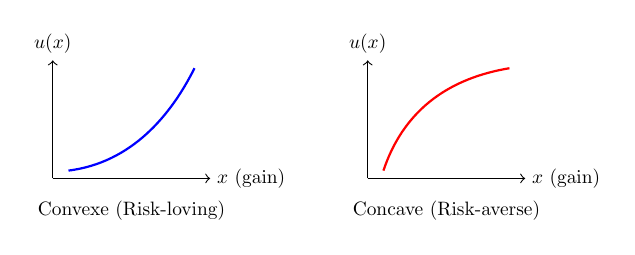
\begin{tikzpicture}[scale=1]
    % Graphique Convexe
    \begin{scope}[shift={(0,0)}]
        \draw[->] (0,0) -- (2,0) node[right, scale=0.7] {$x$ (gain)};
        \draw[->] (0,0) -- (0,1.5) node[above, scale=0.7] {$u(x)$};
        \draw[thick, blue] (0.2,0.1) .. controls (1,0.2) and (1.5,0.8) .. (1.8,1.4);
        \node[below, scale=0.7] at (1,-0.2) {Convexe (Risk-loving)};
    \end{scope}

    % Graphique Concave
    \begin{scope}[shift={(4,0)}]
        \draw[->] (0,0) -- (2,0) node[right, scale=0.7] {$x$ (gain)};
        \draw[->] (0,0) -- (0,1.5) node[above, scale=0.7] {$u(x)$};
        \draw[thick, red] (0.2,0.1) .. controls (0.5,1) and (1.2,1.3) .. (1.8,1.4);
        \node[below, scale=0.7] at (1,-0.2) {Concave (Risk-averse)};
    \end{scope}
\end{tikzpicture}
\\[0.5em]
\textsc{Figure 26} – Fonctions d'utilité convexe (aimant le risque) et concave (averse au risque)
\end{center}
\end{exemple}

\section{Convergences de Suites de Variables Aléatoires}

Soit $(X_n)_{n \in \mathbb{N}}$ une suite de variables aléatoires et $X$ une autre variable aléatoire. Sauf indication contraire, elles sont toutes définies sur le même espace probabilisé $(\Omega, \mathcal{A}, P)$. La convergence en distribution est une exception et ne requiert pas que les v.a. soient sur le même espace.

\subsection{Convergence en Distribution (ou en Loi)}

Notée $X_n \xrightarrow{d} X$ ou $X_n \xrightarrow{\mathcal{L}} X$.

\begin{definition}
La suite $(X_n)_{n \in \mathbb{N}}$ \textbf{converge en distribution} (ou en loi) vers $X$ si :
\[ \lim_{n \to \infty} F_{X_n}(x) = F_X(x) \]
en tout point $x \in \mathbb{R}$ où la fonction de répartition $F_X$ de $X$ est continue.
\end{definition}

\begin{exemple}($X_n = \max(U_1, \dots, U_n)$ avec $U_i \sim \mathcal{U}([0, a])$ i.i.d)

$F_U(x) = x/a$ pour $x \in [0, a]$.\\
$F_{X_n}(x) = P(\max(U_i) \le x) = P(U_1 \le x, \dots, U_n \le x) = (F_U(x))^n = (x/a)^n$ pour $x \in [0, a]$.
\end{exemple}

\noindent Ailleurs, $F_{X_n}(x) = 0$ si $x < 0$ et $F_{X_n}(x) = 1$ si $x > a$. Quand $n \to \infty$ : Si $0 \le x < a$, alors $x/a < 1$, donc $(x/a)^n \to 0$. Si $x = a$, alors $(a/a)^n = 1^n \to 1$. Si $x > a$, $F_{X_n}(x) = 1 \to 1$. Si $x < 0$, $F_{X_n}(x) = 0 \to 0$. Donc, $\lim_{n \to \infty} F_{X_n}(x) = F_a(x) = \begin{cases} 0 & \text{si } x < a \\ 1 & \text{si } x \ge a \end{cases}$. C'est la fonction de répartition d'une variable aléatoire constante égale à $a$. Ainsi, $X_n \xrightarrow{d} a$.

\begin{proposition}[Propriétés de la convergence en distribution]
Soit $X_n \xrightarrow{d} X$.
\begin{enumerate}
    \item \textbf{Théorème de Portmanteau (une implication) / Théorème de la continuité de l'espérance :} Si $f : \mathbb{R} \to \mathbb{R}$ est une fonction continue et \textbf{bornée}, alors $\mathbb{E}[f(X_n)] \xrightarrow[n \to \infty]{} \mathbb{E}[f(X)]$.
    \item \textbf{Continuous Mapping Theorem (CMT) :} Si $g : \mathbb{R} \to \mathbb{R}$ est une fonction continue (plus précisément, continue en dehors d'un ensemble $D_g$ de points de discontinuité tel que $P(X \in D_g) = 0$), alors $g(X_n) \xrightarrow{d} g(X)$.
\end{enumerate}
\end{proposition}

\begin{proposition}[Théoreme de Lévy]
    Nous avons que:
    $X_n \overset{d}{\to}X \Leftrightarrow \varphi_{X_n}(t)\to \varphi_X(t), \quad \forall t\in \R$
\end{proposition}

\begin{remarque}[Limitations de la convergence en distribution]
\begin{enumerate}
    \item Les v.a. $X_n$ et $X$ n'ont pas besoin d'être définies sur le même espace probabilisé.
    \item Si $X_n \xrightarrow{d} X$ et $Y_n \xrightarrow{d} Y$, on n'a pas en général $X_n + Y_n \xrightarrow{d} X + Y$, sauf si une des limites est une constante (voir Lemme de Slutsky).
    \item Le types de problèmes que nous pouvons rencontrer concernant l'unicité de la limite est que pour $X_n \overset{d}{\to}X\sim \operatorname{Unif}{([-1,1])}$ on a aussi $X_n \overset{d}{\to}-X$.
\end{enumerate}
\end{remarque}

\subsection{Convergence en Probabilité}

Notée $X_n \xrightarrow{P} X$. (Nécessite que $X_n$ et $X$ soient sur le même espace probabilisé).

\begin{definition}
La suite $(X_n)_{n \in \mathbb{N}}$ \textbf{converge en probabilité} vers $X$ si pour tout $\varepsilon > 0$ :
$$\lim_{n \to \infty} P(|X_n - X| > \varepsilon) = 0$$
(ou de manière équivalente, $\lim_{n \to \infty} P(|X_n - X| \ge \varepsilon) = 0$).
\end{definition}
Intuitivement la convergence en probabilité  est que pour $n$ grand, la proba que $X_n$ prenne une valeur proche de celle de $X$ est de probabilité $1$.

\begin{exemple}[{Suite de $X_n = \max(U_i)$ avec $U_i \sim \mathcal{U}([0,a])$}]

On a vu $X_n \xrightarrow{d} a$. Montrons que $X_n \xrightarrow{P} a$. Pour $0 < \varepsilon < a$ :
\[
P(|X_n - a| > \varepsilon) = P(a - X_n > \varepsilon) = P(X_n < a - \varepsilon)
= F_{X_n}(a - \varepsilon) = \left(\frac{a-\varepsilon}{a}\right)^n .
\]
Comme $0 < \frac{a-\varepsilon}{a} < 1$, on a $\lim_{n \to \infty} \left(\frac{a-\varepsilon}{a}\right)^n = 0$. Donc $X_n \xrightarrow{P} a$.
\end{exemple}

\begin{proposition}[Propriétés de la convergence en probabilité]
Soit $X_n \xrightarrow{P} X$ et $Y_n \xrightarrow{P} Y$.
\begin{enumerate}
    \item \textbf{Unicité de la limite (p.s.) :} Si $X_n \xrightarrow{P} X$ et $X_n \xrightarrow{P} X'$, alors $X = X'$ p.s.
    \item \textbf{Stabilité par opérations algébriques (Lemme de Slutsky partiel) :} $X_n + Y_n \xrightarrow{P} X + Y$, $X_n Y_n \xrightarrow{P} XY$. Si $Y \neq 0$ p.s., $X_n / Y_n \xrightarrow{P} X/Y$.
    \item \textbf{Continuous Mapping Theorem (CMT) :} Si $g : \mathbb{R} \to \mathbb{R}$ est continue, alors $g(X_n) \xrightarrow{P} g(X)$.
\end{enumerate}
\end{proposition}

\subsection{Convergence Presque Sûre}

Notée $X_n \xrightarrow{p.s.} X$ ou $X_n \xrightarrow{a.s.} X$. (Nécessite $X_n, X$ sur le même espace).

\begin{definition}
La suite $(X_n)_{n \in \mathbb{N}}$ \textbf{converge presque sûrement} vers $X$ si :
$$P(\{\omega \in \Omega \mid \lim_{n \to \infty} X_n(\omega) = X(\omega)\}) = 1$$
C'est la convergence de la suite de fonctions $X_n(\cdot)$ vers $X(\cdot)$ sur un ensemble de mesure 1.
\end{definition}

Une condition suffisante, via le premier lemme de Borel-Cantelli, est : Si $\sum_{n=1}^{\infty} P(|X_n - X| > \varepsilon) < \infty$ pour tout $\varepsilon > 0$, alors $X_n \xrightarrow{p.s.} X$.

\begin{exemple}(Suite de $X_n = \max(U_i)$ avec $U_i \sim \mathcal{U}([0, a])$)
On a $P(|X_n - a| > \varepsilon) = \left(\frac{a-\varepsilon}{a}\right)^n$. La série $\sum_{n=1}^{\infty} \left(\frac{a-\varepsilon}{a}\right)^n$ est une série géométrique de raison $r = \frac{a-\varepsilon}{a} \in [0, 1[$. Elle converge. Par la condition de Borel-Cantelli, $X_n \xrightarrow{p.s.} a$.
\end{exemple}

\begin{proposition}[(Propriétés de la convergence presque sûre)]
Unicité de la limite (p.s.). Stabilité par opérations algébriques. CMT si $g$ continue : $g(X_n) \xrightarrow{p.s.} g(X)$.
\end{proposition}

\begin{proposition}
    Si $\forall \varepsilon>0 : \quad \sum_{n=1}^\infty P(|X_n-X|> \varepsilon)< \infty$ alors $X_n \overset{\text{p.s}}{\to}X$
\end{proposition}

\begin{proof}
    Soit $\varepsilon>0$, Notons $A_n(\varepsilon)=\{\omega\in \Omega\mid |X_n(\omega)-X(\omega)|>\varepsilon\}$. Par hypothèse $\sum_{n=1}^\infty P(|X_n-X|> \varepsilon)< \infty$ et en utilisant Borel-Cantelli 
    \begin{align*}
        &P(\limsup A_n(\varepsilon))=0\\
        =&\bigcap_{n=1}^\infty\bigcup_{k=n}^\infty A_k(\varepsilon)\\
        =&\{\omega\in \Omega \mid \forall n\geq 1, \exists k\ge n: |X_n(\omega)-X(\omega)|>\varepsilon\}
    \end{align*}
    Donc on déduit:
    \[
    \bigcup_{\ell=1}^\infty\bigcap_{n=1}^\infty\bigcup_{k=n}^\infty A_k\left(\frac{1}{\ell}\right)\leq \sum_{\ell=1}^\infty P\left(\bigcap_{n=1}^\infty\bigcup_{k=n}^\infty A_k(\frac{1}{\ell})\right)=0
    \]
    Et le premier membre de l'inégalité est simplement $\{\omega\in \Omega\mid X_n(\omega)\to X(\omega)\}$
\end{proof}

\subsection {Convergence en Moyenne (d'ordre $r$ ou en $L^r$)}

Notée $X_n \xrightarrow{L^r} X$. (Nécessite $X_n, X$ sur le même espace).

\begin{definition}
Soit $r \ge 1$. La suite $(X_n)_{n \in \mathbb{N}}$ \textbf{converge en moyenne d'ordre $r$} vers $X$, si $\mathbb{E}[|X_n|^r] < \infty$ pour tout $n$, $\mathbb{E}[|X|^r] < \infty$, et :
$$\lim_{n \to \infty} \mathbb{E}[|X_n - X|^r] = 0$$
\end{definition}

Cas importants :
\begin{itemize}
    \item $r = 1$ : Convergence en moyenne. $\lim_{n \to \infty} \mathbb{E}[|X_n - X|] = 0$.
    \item $r = 2$ : Convergence en moyenne quadratique. $\lim_{n \to \infty} \mathbb{E}[(X_n - X)^2] = 0$.
\end{itemize}

\begin{exemple}(Suite de $X_n = \max(U_i)$ avec $U_i \sim \mathcal{U}([0, a])$)
Calcul de $\mathbb{E}[X_n] = \frac{na}{n+1}$. $\mathbb{E}[|X_n - a|] = \mathbb{E}[a - X_n]$ (car $X_n \le a$) $= a - \mathbb{E}[X_n] = a - \frac{na}{n+1} = \frac{a}{n+1}$. Comme $\lim_{n \to \infty} \frac{a}{n+1} = 0$, on a $X_n \xrightarrow{L^1} a$.
\end{exemple}

L'idée ici est que, $L^r(\Omega,\A, P):= \{v.a \: X \text{ sur } (\Omega,\A, P)\mid E[|X|^n]<\infty\}$ est un espace vectoriel.
et $|X|_r= (E[|X|^2])^{1/2}$ est une "norme" sur $L^r(\Omega,\A, P)$ alors $L^r$ est la convergence pour cette norme donc les propriétés de base de la limite sont vérifiés.
\section{Comparaisons des modes de convergence}

Voici les principales implications entre les modes de convergence :

\begin{itemize}
    \item \textbf{Convergence presque sûre $\implies$ Convergence en probabilité :} $X_n \xrightarrow{p.s.} X \implies X_n \xrightarrow{P} X$.
    \item \textbf{Convergence en moyenne $L^r$ ($r \ge 1$) $\implies$ Convergence en probabilité :} $X_n \xrightarrow{L^r} X \implies X_n \xrightarrow{P} X$. (Se démontre avec l'inégalité de Markov appliquée à $|X_n - X|^r$).
    \item \textbf{Convergence en probabilité $\implies$ Convergence en distribution :} $X_n \xrightarrow{P} X \implies X_n \xrightarrow{d} X$.
    \item \textbf{Convergence en moyenne $L^r \implies$ Convergence en moyenne $L^s$ (pour $r \ge s \ge 1$) :} Si $X_n \xrightarrow{L^r} X$, alors $X_n \xrightarrow{L^s} X$ pour tout $1 \le s \le r$. (Par l'inégalité de Lyapounov ou Jensen).
\end{itemize}

Les réciproques sont généralement fausses sans conditions supplémentaires. Quelques réciproques (ou liens supplémentaires) notables :

\begin{itemize}
    \item Si $X_n \xrightarrow{d} c$ (où $c$ est une constante), alors $X_n \xrightarrow{P} c$. (Partie du Lemme de Slutsky).
    \item Si $X_n \xrightarrow{P} X$, alors il existe une sous-suite $(X_{n_k})_{k \in \mathbb{N}}$ telle que $X_{n_k} \xrightarrow{p.s.} X$.
    \item Si $X_n \xrightarrow{P} X$ et la suite $(X_n)$ est dominée par une variable aléatoire $Y \in L^r$ (c'est-à-dire $|X_n| \le Y$ p.s. pour tout $n$, et $\mathbb{E}[Y^r] < \infty$), alors $X_n \xrightarrow{L^r} X$. (Conséquence du Théorème de la convergence dominée de Lebesgue).
\end{itemize}

\begin{proposition}
    Si une suite converge en proba alors il existe une sous-suite qui converge presque surement.
\end{proposition}
\section{Fonction Caractéristique}

La fonction caractéristique est un outil puissant en probabilités, notamment pour étudier les sommes de variables aléatoires indépendantes et pour prouver la convergence en distribution (comme dans le TCL).

\begin{definition}[(Fonction caractéristique)]
Soit $X$ une variable aléatoire réelle. Sa \textbf{fonction caractéristique} est une fonction $\varphi_X : \mathbb{R} \to \mathbb{C}$ (à valeurs complexes) définie par :
$$\varphi_X(t) = \mathbb{E}[e^{itX}] = \mathbb{E}[\cos(tX) + i\sin(tX)] = \mathbb{E}[\cos(tX)] + i\mathbb{E}[\sin(tX)]$$
\end{definition}

\noindent où $i^2 = -1$ et $t \in \mathbb{R}$. La fonction caractéristique existe toujours pour toute variable aléatoire, car $|e^{itX}| = 1$, donc $\mathbb{E}[|e^{itX}|] = \mathbb{E}[1] = 1 < \infty$.

\begin{remarque}[Propriétés de la fonction caractéristique]
\begin{enumerate}
    \item $\varphi_X(0) = \mathbb{E}[e^{i \cdot 0 \cdot X}] = \mathbb{E}[1] = 1$.
    \item $|\varphi_X(t)| = |\mathbb{E}[e^{itX}]| \le \mathbb{E}[|e^{itX}|] = \mathbb{E}[1] = 1$. La fonction caractéristique est bornée par 1.
    \item $\varphi_X(-t) = \mathbb{E}[e^{-itX}] = \mathbb{E}[\overline{e^{itX}}] = \overline{\mathbb{E}[e^{itX}]} = \overline{\varphi_X(t)}$ (conjugué complexe).
    \item Transformation affine : $\varphi_{aX+b}(t) = \mathbb{E}[e^{it(aX+b)}] = \mathbb{E}[e^{itaX}e^{itb}] = e^{itb}\mathbb{E}[e^{i(at)X}] = e^{itb}\varphi_X(at)$.
    \item La fonction caractéristique $\varphi_X(t)$ est uniformément continue sur $\mathbb{R}$.
\end{enumerate}
\end{remarque}

\begin{center}
    51
\end{center}

\begin{enumerate}
    \setcounter{enumi}{5}
    \item \textbf{Lien avec les moments :} Si $\mathbb{E}[|X|^k] < \infty$ pour un entier $k \ge 1$ (i.e., $X$ admet un moment d'ordre $k$), alors $\varphi_X$ est $k$ fois continûment dérivable sur $\mathbb{R}$, et sa $j$-ième dérivée en 0 est liée au $j$-ième moment de $X$ (pour $j \le k$) :
    $$\varphi_X^{(j)}(t) = \mathbb{E}[(iX)^j e^{itX}]$$
    En particulier, en $t=0$ : $\varphi_X^{(j)}(0) = \mathbb{E}[(iX)^j] = i^j \mathbb{E}[X^j]$. Donc, $\mathbb{E}[X^j] = \frac{\varphi_X^{(j)}(0)}{i^j} = (-i)^j \varphi_X^{(j)}(0)$. Par exemple : $\mathbb{E}[X] = \frac{\varphi'_X(0)}{i} = -i\varphi'_X(0)$, et $\mathbb{E}[X^2] = \frac{\varphi''_X(0)}{i^2} = -\varphi''_X(0)$.\\
    Cela permet d'obtenir un développement limité de $\varphi_X(t)$ autour de $t=0$ si les moments existent : Si $\mathbb{E}[|X|^k] < \infty$, alors $\varphi_X(t) = \sum_{j=0}^k \frac{\mathbb{E}[X^j](it)^j}{j!} + o(t^k)$ quand $t \to 0$.
\end{enumerate}

\begin{proposition}[Unicité et Théorème de continuité de Lévy]
\begin{enumerate}
    \item \textbf{Théorème d'unicité :} Deux variables aléatoires $X$ et $Y$ ont la même loi de probabilité (c'est-à-dire $F_X(x) = F_Y(x)$ pour tout $x$) si et seulement si elles ont la même fonction caractéristique ($\varphi_X(t) = \varphi_Y(t)$ pour tout $t \in \mathbb{R}$). La fonction caractéristique caractérise donc la loi.
    \item \textbf{Théorème de continuité de Lévy :} Soit $(X_n)_{n \in \mathbb{N}}$ une suite de variables aléatoires. $X_n \xrightarrow{d} X$ si et seulement si $\varphi_{X_n}(t) \xrightarrow[n \to \infty]{} \varphi_X(t)$ pour tout $t \in \mathbb{R}$ (convergence simple des fonctions caractéristiques), et si la fonction limite $\varphi(t) = \lim \varphi_{X_n}(t)$ est continue en $t=0$ (ce qui est automatiquement vrai si $\varphi(t)$ est elle-même une fonction caractéristique).
\end{enumerate}
\end{proposition}

\begin{proposition}[Fonction caractéristique d'une somme de v.a. indépendantes]
Si $X_1, X_2, \dots, X_n$ sont des variables aléatoires \textbf{mutuellement indépendantes}, alors la fonction caractéristique de leur somme $S_n = X_1 + \dots + X_n$ est le produit de leurs fonctions caractéristiques individuelles :
$$\varphi_{S_n}(t) = \prod_{j=1}^n \varphi_{X_j}(t)$$
\end{proposition}

\begin{exemple}[Fonctions caractéristiques usuelles]
\begin{itemize}
    \item Si $Z \sim \mathcal{N}(0, 1)$, alors $\varphi_Z(t) = e^{-t^2/2}$.
    \item Si $X \sim \mathcal{N}(\mu, \sigma^2)$, alors $X = \sigma Z + \mu$ avec $Z \sim \mathcal{N}(0, 1)$. Donc $\varphi_X(t) = \varphi_{\sigma Z + \mu}(t) = e^{it\mu}\varphi_Z(\sigma t) = e^{it\mu}e^{-(\sigma t)^2/2} = e^{it\mu - \sigma^2 t^2/2}$.
    \item \textbf{Application :} Si $X_1 \sim \mathcal{N}(\mu_1, \sigma_1^2)$ et $X_2 \sim \mathcal{N}(\mu_2, \sigma_2^2)$ sont indépendantes, alors $S = X_1 + X_2$. $\varphi_S(t) = \varphi_{X_1}(t)\varphi_{X_2}(t) = e^{it(\mu_1+\mu_2) - (\sigma_1^2+\sigma_2^2)t^2/2}$. C'est la f.c. d'une $\mathcal{N}(\mu_1 + \mu_2, \sigma_1^2 + \sigma_2^2)$.
\end{itemize}
\end{exemple}

\section{Théorèmes Limites}

\subsection{Théorème Central Limite (TCL) - Version de Lindeberg-Lévy}

Soient $X_1, X_2, \dots$ une suite de variables aléatoires \textbf{indépendantes et identiquement distribuées (i.i.d.)} ayant une espérance commune $\mathbb{E}[X_i] = \mu < \infty$ et une variance commune $\text{Var}(X_i) = \sigma^2 \in (0, \infty)$ (finie et strictement positive). Soit $S_n = X_1 + \dots + X_n$ la somme partielle. Soit $\bar{X}_n = \frac{S_n}{n} = \frac{1}{n}\sum_{i=1}^n X_i$ la moyenne empirique. On a $\mathbb{E}[S_n] = n\mu$, $\text{Var}(S_n) = n\sigma^2$ (par indépendance). Et $\mathbb{E}[\bar{X}_n] = \mu$, $\text{Var}(\bar{X}_n) = \frac{n\sigma^2}{n^2} = \frac{\sigma^2}{n}$.

Le TCL stipule que la somme (ou la moyenne) standardisée (centrée et réduite) converge en distribution vers une loi normale centrée réduite :
$$Z_n = \frac{S_n - \mathbb{E}[S_n]}{\sqrt{\text{Var}(S_n)}} = \frac{S_n - n\mu}{\sigma\sqrt{n}} \xrightarrow{d} \mathcal{N}(0, 1)$$

De manière équivalente pour la moyenne empirique :
$$\frac{\bar{X}_n - \mathbb{E}[\bar{X}_n]}{\sqrt{\text{Var}(\bar{X}_n)}} = \frac{\bar{X}_n - \mu}{\sigma/\sqrt{n}} \xrightarrow{d} \mathcal{N}(0, 1)$$

Cela signifie que pour $n$ suffisamment grand, la distribution de $S_n$ peut être approximée par une loi $\mathcal{N}(n\mu, n\sigma^2)$, et celle de $\bar{X}_n$ par une loi $\mathcal{N}(\mu, \sigma^2/n)$.

\begin{remarque}[Idée de la preuve du TCL via les fonctions caractéristiques]
Pour simplifier, on suppose $X_i$ i.i.d. avec $\mathbb{E}[X_i] = 0$ et $\text{Var}(X_i) = 1$ (sinon, on travaille avec $Y_i = (X_i - \mu)/\sigma$). Alors $\mathbb{E}[X_i^2] = 1$. On s'intéresse à $Z_n = \frac{S_n}{\sqrt{n}} = \sum_{i=1}^n \frac{X_i}{\sqrt{n}}$. 

$\varphi_{Z_n}(t) = \mathbb{E}[e^{itS_n/\sqrt{n}}] = \mathbb{E}[\prod_{i=1}^n e^{itX_i/\sqrt{n}}] = \prod_{i=1}^n \mathbb{E}[e^{itX_i/\sqrt{n}}]$ (par indépendance). Comme les $X_i$ sont i.i.d., $\varphi_{X_i/\sqrt{n}}(t) = \varphi_{X_1}(t/\sqrt{n})$. Donc $\varphi_{Z_n}(t) = (\varphi_{X_1}(t/\sqrt{n}))^n$. 

On utilise le développement limité de $\varphi_{X_1}(u)$ autour de $u=0$ à l'ordre 2 (car $\mathbb{E}[X_1]=0, \mathbb{E}[X_1^2]=1$) : 
$\varphi_{X_1}(u) = \varphi_{X_1}(0) + u\varphi'_{X_1}(0) + \frac{u^2}{2}\varphi''_{X_1}(0) + o(u^2) = 1 + u(i\mathbb{E}[X_1]) + \frac{u^2}{2}(i^2\mathbb{E}[X_1^2]) + o(u^2) = 1 + 0 - \frac{u^2}{2} + o(u^2)$. 

En posant $u = t/\sqrt{n} : \varphi_{X_1}(t/\sqrt{n}) = 1 - \frac{(t/\sqrt{n})^2}{2} + o((t/\sqrt{n})^2) = 1 - \frac{t^2}{2n} + o(1/n)$. 

Alors $\varphi_{Z_n}(t) = \left( 1 - \frac{t^2}{2n} + o(1/n) \right)^n$. En utilisant le fait que si $a_n \to a$, alors $(1 + a_n/n)^n \to e^a$. Ici, avec $a_n = -t^2/2 + n \cdot o(1/n)$, on a $a_n \to -t^2/2$. 

Donc $\lim_{n \to \infty} \varphi_{Z_n}(t) = e^{-t^2/2}$. C'est la fonction caractéristique d'une loi $\mathcal{N}(0, 1)$. Par le théorème de continuité de Lévy, $Z_n \xrightarrow{d} \mathcal{N}(0, 1)$. \hfill $\square$
\end{remarque}

\subsection{Loi Faible des Grands Nombres (LFGN)}

Soient $X_1, X_2, \dots$ une suite de variables aléatoires i.i.d. avec une espérance commune $\mathbb{E}[X_i] = \mu < \infty$. (La loi faible des grands nombres ne requiert pas de variance finie). Alors la moyenne empirique $\bar{X}_n = \frac{1}{n} \sum_{i=1}^n X_i$ converge en probabilité vers $\mu$ :
$$\bar{X}_n \xrightarrow{P} \mu$$
C'est-à-dire, pour tout $\varepsilon > 0, \lim_{n \to \infty} P(|\bar{X}_n - \mu| > \varepsilon) = 0$.

\begin{proof}
(Dans le cas où $\text{Var}(X_i) = \sigma^2 < \infty$ existe pour tout $i$). On a $\mathbb{E}[\bar{X}_n] = \mu$ et $\text{Var}(\bar{X}_n) = \frac{1}{n^2} \text{Var}(\sum X_i) = \frac{1}{n^2} \sum \text{Var}(X_i) = \frac{n\sigma^2}{n^2} = \frac{\sigma^2}{n}$. Par l'inégalité de Bienaymé-Tchebychev appliquée à $\bar{X}_n$ :
$$P(|\bar{X}_n - \mathbb{E}[\bar{X}_n]| \ge \varepsilon) \le \frac{\text{Var}(\bar{X}_n)}{\varepsilon^2}$$
$$P(|\bar{X}_n - \mu| \ge \varepsilon) \le \frac{\sigma^2/n}{\varepsilon^2} = \frac{\sigma^2}{n\varepsilon^2}$$
Quand $n \to \infty$, $\frac{\sigma^2}{n\varepsilon^2} \to 0$ (car $\sigma^2$ et $\varepsilon^2$ sont fixes et finis). Donc $\lim_{n \to \infty} P(|\bar{X}_n - \mu| \ge \varepsilon) = 0$. D'où $\bar{X}_n \xrightarrow{P} \mu$.
\end{proof}

\begin{proof}[en cours]
    Soit $\varepsilon>0$. On veut montrer que $P(|\overline{X}^n-\mu|> \varepsilon)\to 0$, on a 
    \begin{align*}
        E&=E[\frac{1}{n}\sum_{i=1}^n X_i]\\
        &=\frac{1}{n}\sum_{i=1}^n E[X_i]\\
        &= \mu
    \end{align*}
    et pour la variance $\Var[\overline{X}^n]= \frac{\sigma^2}{n}$ Puis inégalité hop hop
\end{proof}

\vspace{1em}

\begin{exemple}[Jeu de Casino et TCL/LFGN]
Considérons un jeu de casino où un joueur gagne $1$ euro avec probabilité $p$ et perd $1$ euro avec probabilité $1-p$. Soit $X_i$ le gain à la $i$-ème partie.
$\mathbb{E}[X_i] = 1 \cdot p + (-1) \cdot (1-p) = 2p-1$. $\mathbb{E}[X_i^2] = 1^2 \cdot p + (-1)^2 \cdot (1-p) = 1$. $\text{Var}(X_i) = \mathbb{E}[X_i^2] - (\mathbb{E}[X_i])^2 = 1 - (2p-1)^2 = 4p(1-p)$. Notons $\mu = 2p-1$ et $\sigma^2 = 4p(1-p)$. Si $p < 1/2$, alors $\mu < 0$. La LFGN indique que $\bar{X}_n = S_n/n \xrightarrow{P} \mu < 0$, donc en moyenne, le joueur perd. Pour $n$ grand, quelle est la probabilité que le gain total $S_n$ soit non négatif, $P(S_n \ge 0)$ ? Par le TCL, $Z_n = \frac{S_n-n\mu}{\sigma\sqrt{n}} \approx Z \sim \mathcal{N}(0,1)$.

$$P(S_n \ge 0) = P\left( \frac{S_n - n\mu}{\sigma\sqrt{n}} \ge \frac{0 - n\mu}{\sigma\sqrt{n}} \right)$$
$$\approx P\left( Z \ge -\frac{\sqrt{n}\mu}{\sigma} \right) = 1 - \Phi\left( -\frac{\sqrt{n}\mu}{\sigma} \right)$$

Puisque $\mu < 0$, le terme $-\frac{\sqrt{n}\mu}{\sigma}$ est positif et tend vers $+\infty$ quand $n \to \infty$. Donc $\Phi\left( -\frac{\sqrt{n}\mu}{\sigma} \right) \to 1$, et $P(S_n \ge 0) \to 0$. \textbf{Application numérique} : Si $p = 0.45$ et $n = 100$. $\mu = 2(0.45)-1 = -0.1$. $\sigma^2 = 4(0.45)(0.55) = 0.99 \implies \sigma \approx 0.995$. La borne devient $\frac{\sqrt{100}(-0.1)}{0.995} = \frac{10 \times 0.1}{0.995} \approx 1.005$. $P(S_{100} \ge 0) \approx 1 - \Phi(1.005) \approx 1 - 0.8425 \approx 0.1575 \approx 0.16$.
\end{exemple}

\subsubsection*{Loi Forte des Grands Nombres (LFFGN)}

Soient $X_1, X_2, \dots$ une suite de variables aléatoires i.i.d. avec une espérance commune $\mathbb{E}[X_i] = \mu < \infty$. Alors la moyenne empirique $\bar{X}_n = \frac{1}{n} \sum_{i=1}^n X_i$ converge presque sûrement vers $\mu$ :
$$\bar{X}_n \xrightarrow{p.s.} \mu$$
C'est-à-dire $P(\lim_{n \to \infty} \bar{X}_n = \mu) = 1$. La convergence presque sûre est une condition plus forte que la convergence en probabilité.

\begin{exemple}[Interprétation fréquentiste de la probabilité]
Soit $A$ un événement associé à une expérience aléatoire, et $P(A)$ sa probabilité. On répète l'expérience $n$ fois de manière indépendante. Soit $X_i = \mathbf{1}_A$ se réalise à l'essai $i$ (variable indicatrice). Alors $X_i \sim \text{Bernoulli}(P(A))$, et $\mathbb{E}[X_i] = P(A)$. La moyenne empirique $\bar{X}_n = \frac{1}{n} \sum_{i=1}^n X_i$ est la fréquence observée de l'événement $A$ sur $n$ essais. Par la LFFGN, $\bar{X}_n \xrightarrow{p.s.} \mathbb{E}[X_i] = P(A)$. La fréquence empirique de réalisation d'un événement converge (presque sûrement) vers sa probabilité théorique lorsque le nombre d'essais tend vers l'infini.
\end{exemple}


Preuve cool 
\begin{proof}
    On peut supposer spdg $\mu= 0$ sinon $X'_i= X_i-\mu$. On va montrer que $(\overline{X}^n)^4$ converge p.s vers 0. On va montrer que $\forall \epsilon>0$ 
    \[
    \sum_{n=1}^\infty P(|(\overline{X}^n)^4|>\varepsilon)<\infty
    \]
    On a 
    \begin{align*}
        E[(\overline{X}^n)^4]&= \frac{1}{n^4}E[(X_i+\cdots + X_n)(X_i+\cdots + X_n)(X_i+\cdots + X_n)(X_i+\cdots + X_n)]\\
        &=\frac{1}{n^4}\left(nE[X_i^4]+ {n\choose 2} {4 \choose 2} E[X^2_i]^2\right)\\
        &=\frac{1}{n^4}\left( na+3bn(n-1)\right)\\
        &\le\frac{Cn^2}{n^4}\\
        &=\frac{C}{n^2}  
    \end{align*}
    Par inégalité de Markov, on obtient que 
    \begin{equation*}
        P(|(\overline{X}^n)^4|>\varepsilon)\le \frac{E[|(\overline{X}^n)^4|]}{\varepsilon}\le \frac{c}{\varepsilon n^2}
    \end{equation*}
    Par critère de comparaison avec la suite $\left(\frac{c}{\varepsilon n^2}\right)$. Ce qui montre que $\sum_{n>0}P(|(\overline{X}^n)^4|>\varepsilon)$ converge. Ceci conclut la preuve
\end{proof}

\subsection{Théorème central limite}
\begin{theoreme}[Central limite]
    $X_1,X_2,...$ iid avec $E[X_i]= \mu$ et $\Var[X_i]= \sigma^2 < \infty$ Alors

    \[
    \frac{\sqrt{n}}{\sigma}(\overline{X}^{(n)}- \mu) \overset{d}{\longrightarrow} \mathcal{N}(0,1)
    \]
    Autrement dit pour $n$ grand,
    \[\overline{X}^{(n)}\approx \mathcal{N}(\mu, \frac{\sigma^2}{n}) \]
\end{theoreme}

\begin{proof}[sans arnaques (nouvelles)]
    On note $Z_n= \frac{\sqrt{n}}{\sigma}(\overline{X}^{(n)}-\mu)=\frac{\sqrt{n}}{\sigma}(\frac{1}{n}\sum X_i-\frac 1 n \sum \mu)$, donc 
    \[
    Z_n=\frac 1 {\sqrt{n}}  \sum_{i=1}^n \frac{X_i- \mu}{\sigma}=  \frac 1 {\sqrt{n}}  \sum_{i=1}^n Y_i
    \]
    où $E[Y_i]= 0$ et $\Var [Y_i]= 1$. On a 

\begin{align*}
    \varphi_{Z_n}(t)&= E\left[e^{i\frac{t}{\sqrt n}\sum_{i=0}^n Y_i}\right]\\
    &=E\left[e^{\frac{itY_1}{\sqrt{n}}}e^{\frac{itY_2}{\sqrt{n}}}\dots e^{\frac{itY_n}{\sqrt{n}}}\right]\\
    &=E\left[e^{\frac{itY_1}{\sqrt{n}}}\right ] E\left[e^{\frac{itY_2}{\sqrt{n}}}\right] \dots E\left[e^{\frac{itY_n}{\sqrt{n}}}\right]\\
    &=E\left[e^{\frac{itY_1}{\sqrt{n}}}\right]^n\\
    &=\varphi_{Y_1}\left(\frac{1}{\sqrt{n}}\right)^n
\end{align*}
    On a par développement de taylor que $$ \varphi_{Y_1}(t)= 1 - \frac{t^2}{2n} + o(t^2/n)$$
    Et finalement on trouve que \begin{align*}
        \lim_{n\to \infty}\varphi_{Z_n}(t)&=\lim_{n\to +\infty}\left(1 - \frac{t^2}{2n} + o(t^2/n)\right)^n\\
        &=e^{\frac{t^2}{2}}\\
        &=\varphi_Z(t)
    \end{align*}
    ou $Z\sim \mathcal{N}(0,1)$. Par le théorème de Levy , on trouve que $Z_n$ converge en distribution vers $Z$. Ceci conclut la preuve
\end{proof}
